% Unofficial UChicago CS Poster Template
% v1.1.0 released September 8, 2022
% https://github.com/k4rtik/uchicago-poster
% a fork of https://github.com/anishathalye/gemini

\documentclass[final]{beamer}

% ====================
% Packages
% ====================

\usepackage[T1]{fontenc}
\usepackage{lmodern}
% Poster size required by the course: 24" wide x 36" high (portrait).
% 24 in = 60.96 cm, 36 in = 91.44 cm. Lower `scale` if a column overflows.
\usepackage[size=custom,width=60.96,height=91.44,scale=1.0]{beamerposter}
\usetheme{gemini}
\usecolortheme{uchicago}
\usepackage{graphicx}
\usepackage{booktabs}
\usepackage{doi}
\usepackage[numbers]{natbib}
\usepackage[patch=none]{microtype}
\usepackage{tikz}
\usepackage{pgfplots}
\pgfplotsset{compat=1.18}
\usepackage{anyfontsize}

\pdfstringdefDisableCommands{%
\def\translate#1{#1}%
}

% ====================
% Lengths
% ====================

% Two columns for a portrait poster:
% (N+1)*\sepwidth + N*\colwidth = \paperwidth, with N = 2.
\newlength{\sepwidth}
\newlength{\colwidth}
\setlength{\sepwidth}{0.025\paperwidth}
\setlength{\colwidth}{0.4625\paperwidth}

\newcommand{\separatorcolumn}{\begin{column}{\sepwidth}\end{column}}

\newcommand{\rtwo}{\ensuremath{R^2}}

% ====================
% Title
% ====================

\title{What Do Sequential Generative Latents Encode?}

\author{Ricky (Xinrui) Bao}

\institute[UChicago]{Department of Computer Science, University of Chicago}

% ====================
% Footer (optional)
% ====================

\footercontent{
  Probing a DreamerV3 World Model Against a Static VAE \hfill
  University of Chicago --- Final Project Poster \hfill
  \href{mailto:rickybao@uchicago.edu}{rickybao@uchicago.edu}}

% ====================
% Logo (optional)
% ====================

\addtobeamertemplate{headline}{}
{
    \begin{tikzpicture}[remember picture,overlay]
      \node [anchor=north west, inner sep=3cm] at ([xshift=0.0cm,yshift=1.0cm]current page.north west)
      {\includegraphics[height=5.0cm]{logos/uc-logo-white.eps}}; % also try shield-white.eps
      \node [anchor=north east, inner sep=3cm] at ([xshift=0.0cm,yshift=2.5cm]current page.north east)
      {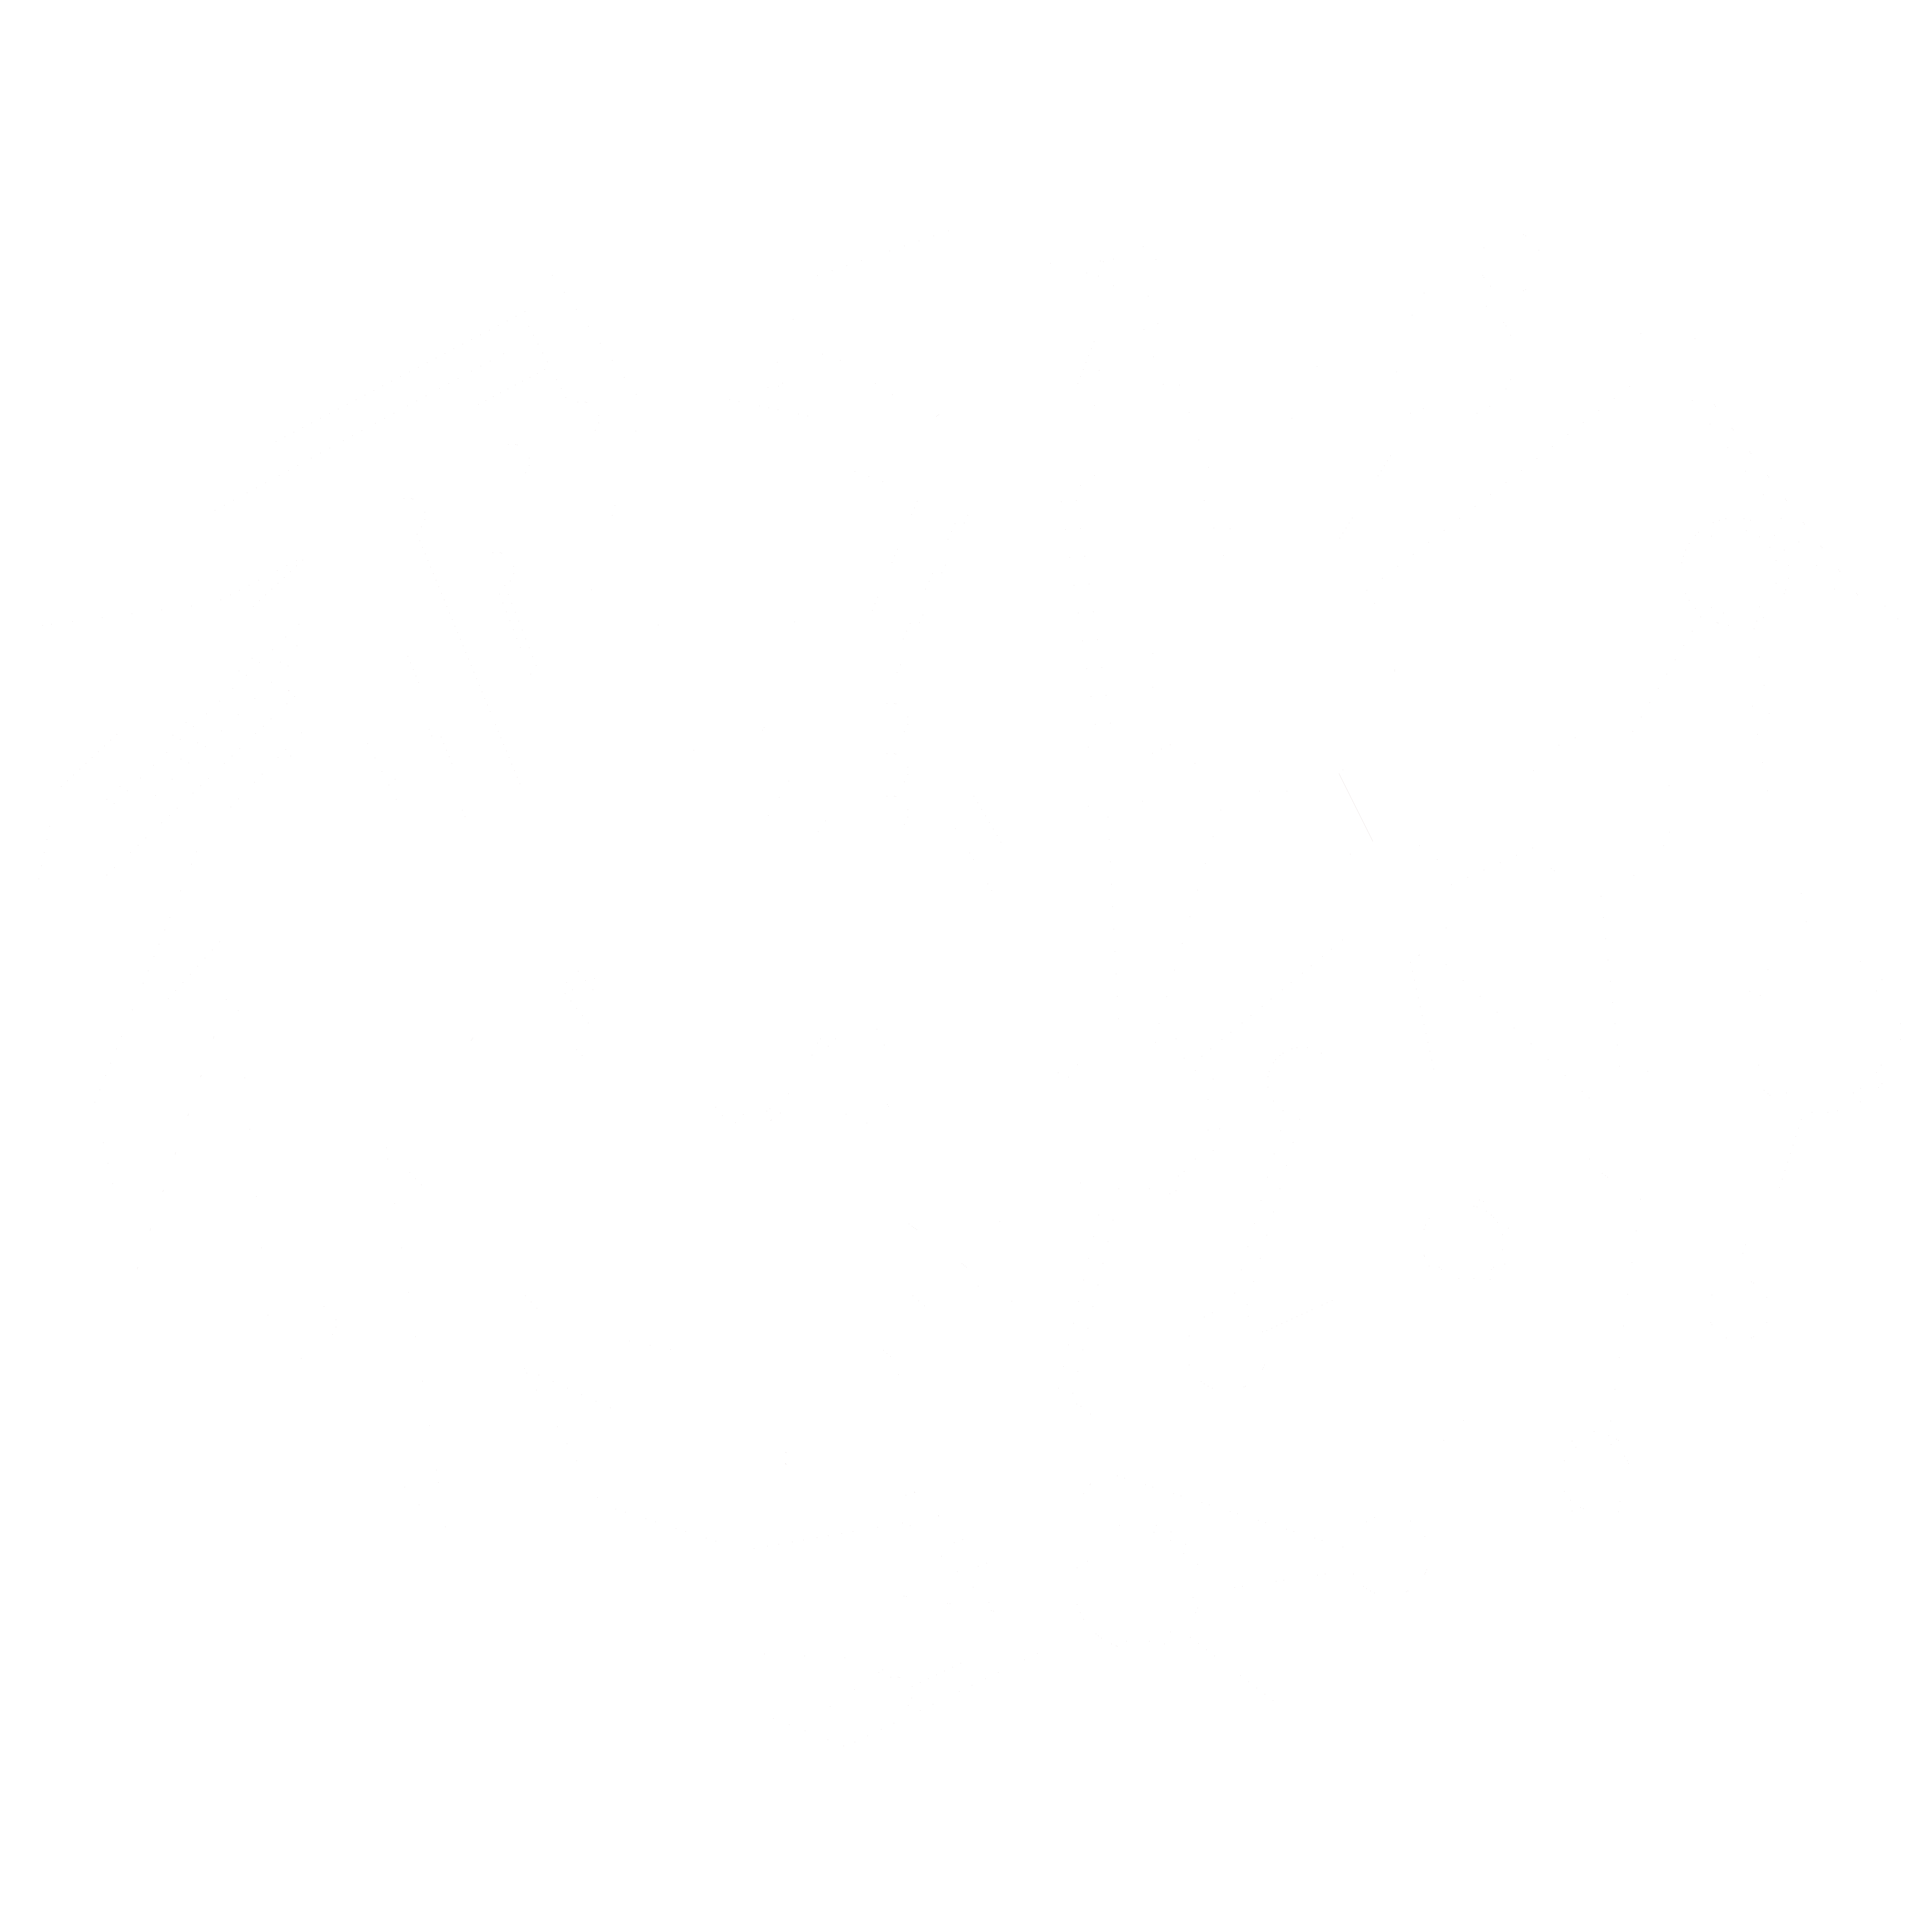
\includegraphics[height=8.0cm]{logos/cs-logo-white.png}};
    \end{tikzpicture}
}

% ====================
% Body
% ====================

\begin{document}

\begin{frame}[t]
\begin{columns}[t]
\separatorcolumn

% ====================================================================
% LEFT COLUMN
% ====================================================================
\begin{column}{\colwidth}

  \begin{block}{Motivation}

    A \textbf{world model} learns a state representation that can be rolled
    forward to predict the future. DreamerV3~\citep{hafner2025dreamerv3} learns
    its representation \emph{sequentially}: a recurrent state-space model (RSSM)
    \citep{hafner2019planet} encodes each observation into a stochastic latent,
    concatenates it with a deterministic recurrent state, and is trained to
    reconstruct observations and predict its own next latent. Unsupervised
    representation learning (e.g.\ a VAE~\citep{kingma2014vae}) is usually
    studied on \emph{static} data instead.

    World-model latents are increasingly reused as pretrained representations
    for control, so what they encode matters. We ask:

    \begin{quote}
      \textbf{What does a sequential generative latent encode beyond a static,
      per-frame model trained on the same observations?}
    \end{quote}

    \textbf{Probing}~\citep{alain2016probes} answers this by measuring how well
    a simple readout recovers a target from a \emph{frozen} representation.
    ST-DIM~\citep{anand2019atari} used the same logic to score Atari
    representations by ground-truth state recovery; we ask a narrower,
    \emph{controlled} sequential-vs-static question.

  \end{block}

  \begin{block}{A controlled comparison}

    We freeze two models and probe both. Fairness controls isolate
    \emph{sequential structure} as the variable of interest:

    \begin{itemize}
      \item \textbf{Same encoder \& decoder architecture} (the VAE is trained
        from scratch, not shared weights).
      \item \textbf{Same observation model} --- a unit-variance Gaussian in
        $\mathrm{symlog}$ space, so held-out likelihoods are comparable.
      \item \textbf{Same training frames} (the DreamerV3 replay buffer).
    \end{itemize}

    The static VAE removes recurrence and dynamics, mapping a single frame to a
    diagonal-Gaussian latent trained on the (negative) ELBO:
    \[
      \mathcal{L}_\beta(x) =
      \underbrace{\mathbb{E}_{q(z\mid x)}\!\big[-\log p(x\mid z)\big]}_{\text{reconstruction}}
      + \beta\,\mathrm{KL}\!\big(q(z\mid x)\,\Vert\,\mathcal{N}(0,I)\big).
    \]

    \textbf{Task \& models:} DeepMind Control proprioceptive Walker-Walk
    \citep{tassa2018dmc}; three DreamerV3 seeds (two to 500K steps, one to
    1.1M) and one matched VAE per seed.

  \end{block}

  \begin{block}{Probing battery}

    For a frozen representation $z$ and target $y$ we fit a probe $g$ and report
    held-out \rtwo{} against the train-mean baseline:
    \[
      R^2 = 1 - \frac{\sum (y-g(z))^2}{\sum (y-\bar y_{\text{train}})^2}.
    \]
    The same \textbf{ridge} (primary) and \textbf{MLP} (robustness) probes are
    used everywhere; splits are by episode.

    \begin{itemize}
      \item \textbf{Targets:} current state; future state at $k\in\{1,5,20\}$;
        gait phase.
      \item \textbf{Sites:} encoder; RSSM posterior ($h_t$, $\mathbb{E}[z_t]$);
        RSSM prior, rolled open-loop $k$ steps on recorded actions; VAE latent.
      \item \textbf{Receptive field:} VAE latent with $K{=}1,4,16,\text{all}$
        causal frames (post-hoc temporal aggregation).
      \item \textbf{Baseline:} a learned forward model
        $g(z_t,a_t)\approx z_{t+1}-z_t$ in the \emph{frozen VAE latent},
        rolled open-loop --- the static analog of the RSSM prior.
    \end{itemize}

  \end{block}

  \begin{block}{Result 1 --- Per-frame current state is shared}

    \begin{figure}
      \centering
      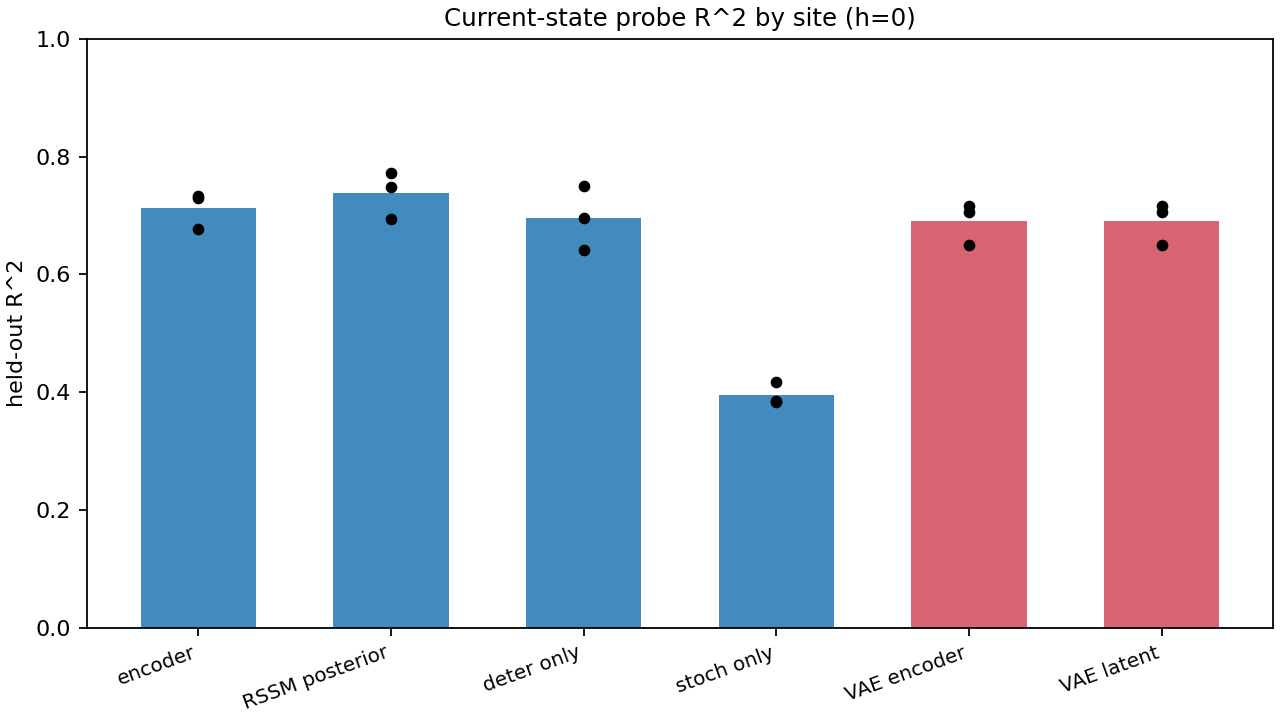
\includegraphics[width=0.78\linewidth]{figures/current_state_probe_r2_by_site.png}
    \end{figure}

    Encoder, RSSM posterior, RSSM deterministic state, and VAE all decode the
    current state at $\rtwo\approx0.69$--$0.74$. Within the RSSM the content
    sits mainly in the \textbf{deterministic state} (0.70); the categorical
    stochastic latent alone is weaker (0.40 linear, 0.55 MLP). At equal width
    the continuous VAE latent (0.69) is the stronger \emph{linear} state code.

  \end{block}

  \begin{block}{Result 2 --- Static pooling closes the gap}

    \begin{figure}
      \centering
      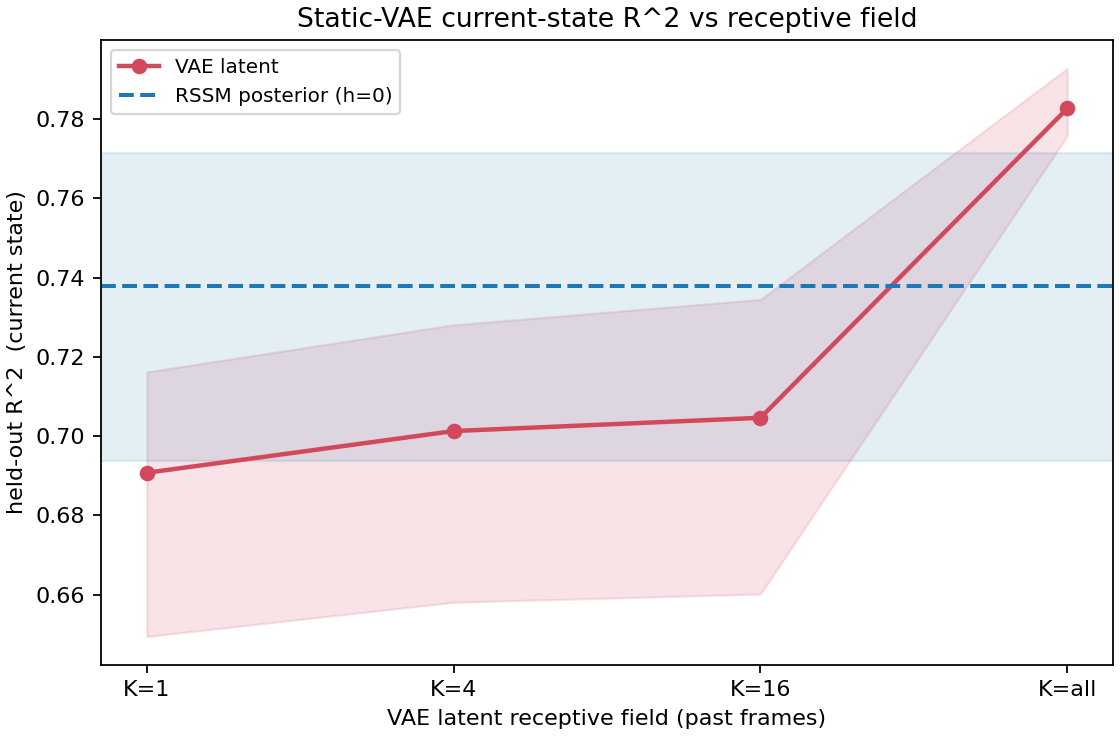
\includegraphics[width=0.78\linewidth]{figures/vae_receptive_field_r2.png}
    \end{figure}

    The VAE's current-state \rtwo{} rises $0.69\!\rightarrow\!0.78$ once it
    includes a causal whole-episode mean, \textbf{overtaking the RSSM
    posterior} (0.74). A handful of recent frames ($K{=}4,16$) is not enough.
    So the current-state content is recoverable from static features by a
    hand-specified temporal summary --- not learned recurrence.

  \end{block}

\end{column}

\separatorcolumn

% ====================================================================
% RIGHT COLUMN
% ====================================================================
\begin{column}{\colwidth}

  \begin{alertblock}{Result 3 --- Prediction lives in the RSSM prior}

    \begin{figure}
      \centering
      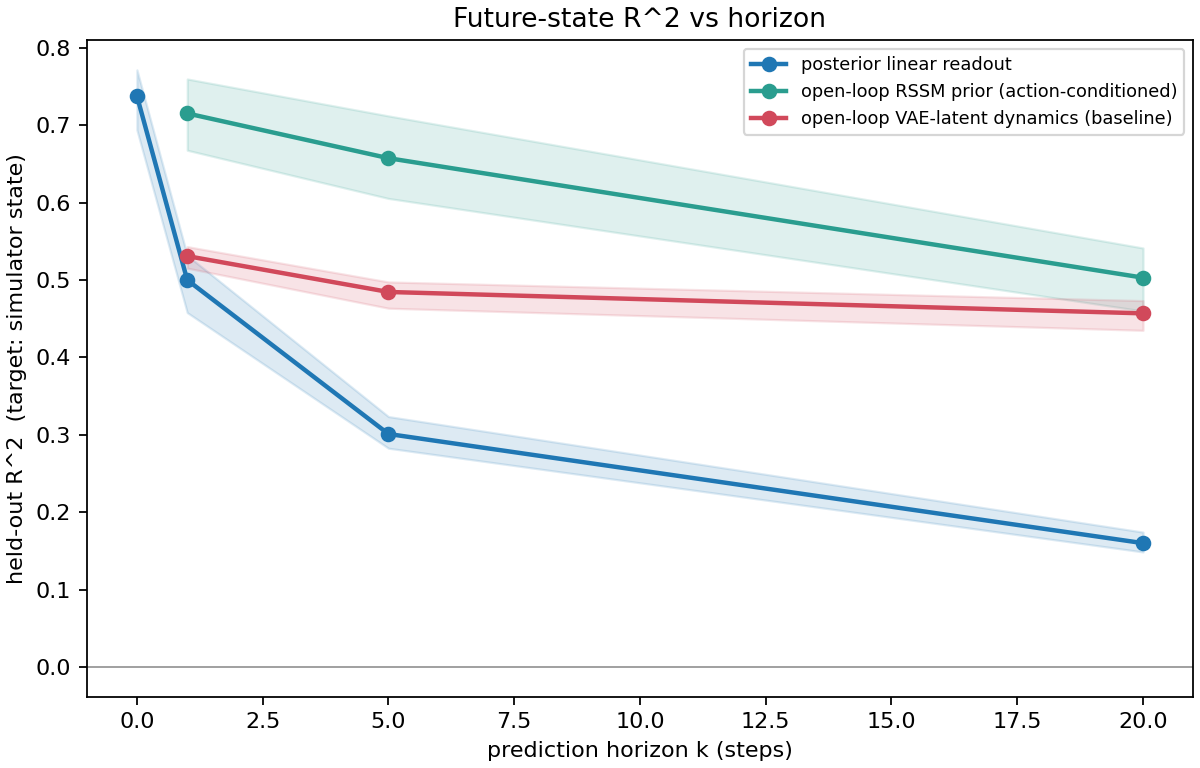
\includegraphics[width=0.78\linewidth]{figures/future_state_r2_by_horizon_posterior_vs_prior.png}
    \end{figure}

    Rolling the \textbf{prior} forward retains far more future state than a
    linear \emph{readout} of the posterior: at $k{=}20$, $\rtwo\approx0.50$ vs
    $0.16$ ($\sim$3$\times$). Giving the static VAE its own learned dynamics is
    a \textbf{strong baseline} (0.46 at $k{=}20$). The RSSM prior still leads
    within every seed under the linear probe, but the margin shrinks with
    horizon ($+0.18$ at $k{=}1 \rightarrow +0.05$ at $k{=}20$) as both reach a
    similar predictability ceiling.

  \end{alertblock}

  \begin{block}{Result 4 --- Gait phase becomes linearly decodable}

    \begin{figure}
      \centering
      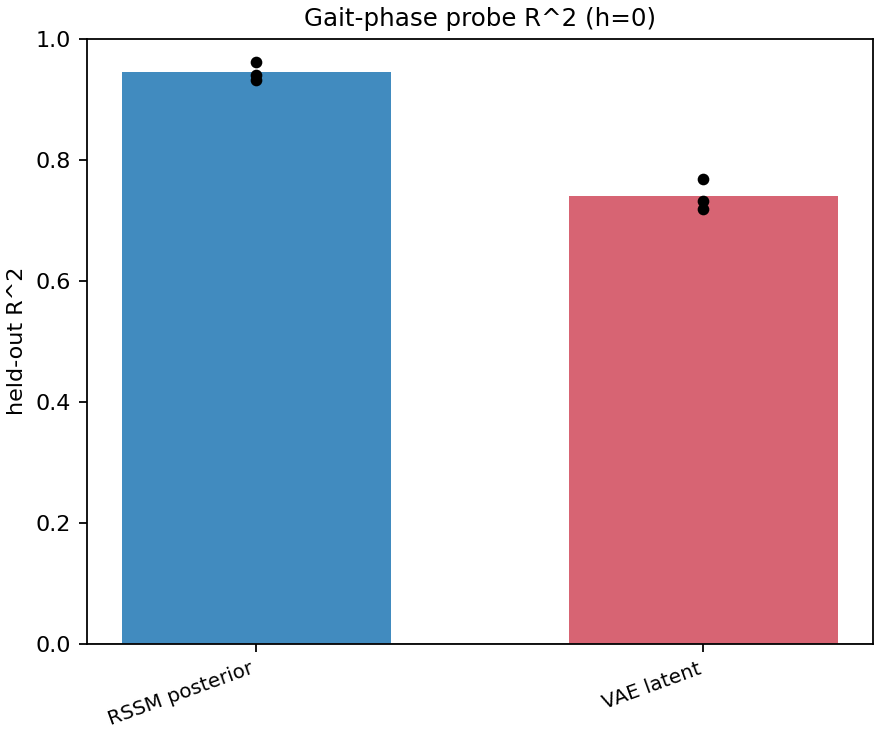
\includegraphics[width=0.62\linewidth]{figures/gait_phase_r2_rssm_vs_vae.png}
    \end{figure}

    Largest linear gap: gait phase decodes at $\rtwo\approx0.95$ from the
    posterior vs $0.74$ from the VAE latent ($+0.21$). A single frame cannot
    place position-within-a-cycle. But an \textbf{MLP} recovers most of it from
    the static latent (0.89 vs 0.95) --- the RSSM mainly makes cyclic structure
    \emph{more linearly accessible}, not newly present.

  \end{block}

  \begin{block}{Result 5 --- Likelihood $\neq$ probe quality}

    \begin{figure}
      \centering
      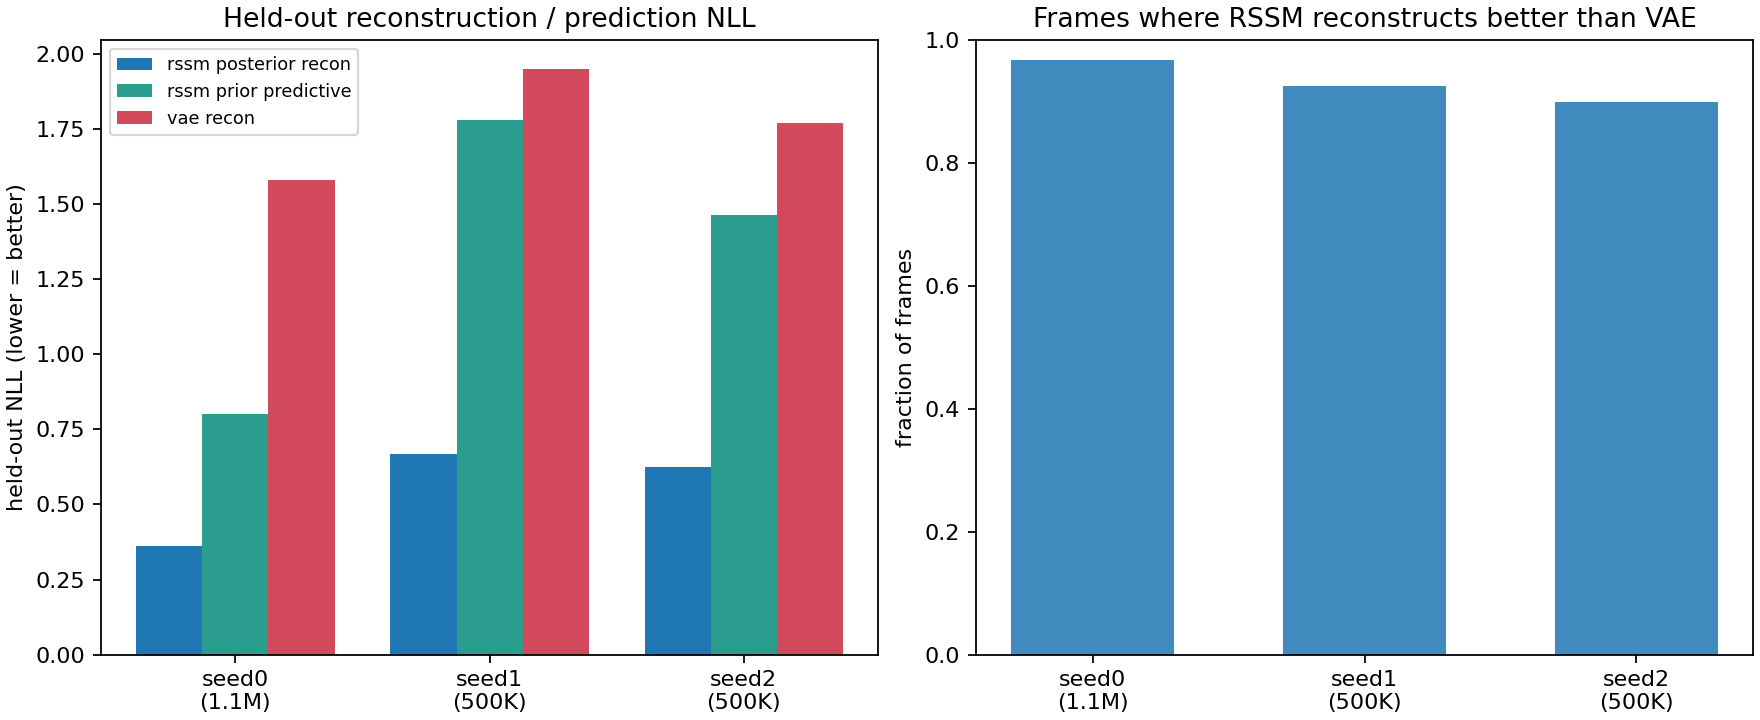
\includegraphics[width=\linewidth]{figures/generative_nll_and_reconstruction_advantage.png}
    \end{figure}

    The RSSM reconstructs with much lower NLL than the VAE (and on 90--97\% of
    frames), and the 1.1M seed lower still --- yet its current-state probe
    \rtwo{} barely moves. \textbf{Reconstruction likelihood and linear
    decodability decouple.}

  \end{block}

  \begin{exampleblock}{Conclusions}

    In near-fully-observed proprioception:
    \begin{itemize}
      \item The sequential latent encodes \textbf{no more current state} than a
        static VAE plus simple causal pooling.
      \item Its value is \textbf{predictive} (action-conditioned prior) and
        \textbf{coordinate-shaping} (linearizes cyclic gait phase).
      \item A static representation \emph{plus learned dynamics} recovers much
        of the predictive content --- recurrence is not required to access it.
      \item Generative likelihood is \textbf{not} a proxy for probe quality.
    \end{itemize}

  \end{exampleblock}

  \begin{block}{Future work}

    \begin{itemize}
      \item \textbf{Pixel / partially observed} tasks, where recurrence should
        matter more for current-state inference.
      \item More seeds and model sizes; a \emph{controlled} training-length
        sweep (only one seed reached 1.1M here).
      \item Per-component (not pooled) probing; stronger VAE-dynamics models.
      \item Does linear accessibility of the latent predict \emph{downstream
        control} transfer?
    \end{itemize}

  \end{block}

  \begin{block}{References}

    \nocite{*}
    \footnotesize{\bibliographystyle{plainnat}\bibliography{poster}}

  \end{block}

\end{column}

\separatorcolumn
\end{columns}
\end{frame}

\end{document}
